\documentclass[11pt, a4paper]{article}
\usepackage[utf8]{inputenc}
\usepackage{geometry}
\geometry{a4paper, margin=0.5in}
\usepackage{titling}
\usepackage{titlesec}
\usepackage{hyperref}
\usepackage{amsmath}
\usepackage{tikz}
\usetikzlibrary{arrows.meta, positioning, shapes.geometric}

\title{\textbf{Final Project Proposal: Refinement-Aware Diverse Trace Selection for Parallel CEGAR}}
\author{Hsu, Chen-Yu(R14943074), Huang, Shao-Chi(R14921035)}
\date{\today}

\begin{document}

\maketitle

\section*{1. Motivation}
Counterexample-Guided Abstraction Refinement (CEGAR) is a widely used framework for software model checking. It repeatedly searches for candidate error traces, checks whether they are semantically feasible, and refines the abstraction when a trace is spurious. Recent work on parallel trace abstraction shows that different candidate traces can be checked in parallel by multiple CPU workers. However, naive parallelization can waste work: several workers may analyze similar traces, and one worker may spend time on a trace that would be pruned by another worker's refinement result. Our motivation is to study refinement-aware parallel CEGAR, where diverse trace selection and a shared refinement cache work together to reduce redundant SMT queries and improve response time.

\section*{2. Problem Formulation}
We formulate software safety verification as reachability over a program automaton $A = (L, \Sigma, \delta, l_0, F_{err})$, where $L$ is the set of program locations, $\Sigma$ is the set of program operations, $\delta$ is the transition relation, $l_0$ is the initial location, and $F_{err}$ is the set of error locations. A candidate counterexample is a syntactic trace $\pi \in \Sigma^*$ that leads from $l_0$ to some error location. For each trace $\pi$, we construct an SSA-based path formula $\Phi_\pi$ and query an SMT solver. If $\Phi_\pi$ is satisfiable, the trace is a real counterexample. If $\Phi_\pi$ is unsatisfiable, the trace is spurious and can be used to refine the search space.

The central problem of this project is not only to parallelize trace checking, but also to reduce redundant parallel work. We maintain a shared refinement cache $R$ containing information learned from spurious traces, such as exact infeasible traces, infeasible prefixes, and optionally unsat-core-based conflict patterns. A trace selector should choose uncovered traces that are diverse from traces already assigned to workers. The verification succeeds with \textsc{Safe} when no uncovered trace to an error location remains, and with \textsc{Unsafe} when any worker finds a satisfiable trace formula.

\section*{3. Method(s) to Try}
We propose a lightweight multi-threaded CEGAR prototype for a simplified imperative language with assignments, assumptions, branches, bounded loops, and assertions. The program is parsed into a CFG, and candidate error traces are generated from the CFG. A coordinator maintains the global trace search state, the set of currently assigned traces, and the shared refinement cache. Worker threads receive traces from the coordinator, check whether they are already covered by the cache, construct SSA formulas for uncovered traces, and use an SMT solver such as Z3 to decide feasibility.

We will compare several trace selection and refinement-sharing strategies. The baseline selector uses ordinary breadth-first search to pick the shortest available error trace. A diverse selector prefers traces that diverge early from traces already assigned to workers, so that workers are less likely to analyze nearly identical counterexamples. A cache-aware selector additionally avoids traces covered by known refinements and prioritizes traces that are expected to add new information. For refinement sharing, we start with exact trace blocking and infeasible-prefix blocking; if time permits, we will add unsat-core-based patterns to generalize refinements beyond one concrete trace.

\begin{figure}[h]
\centering
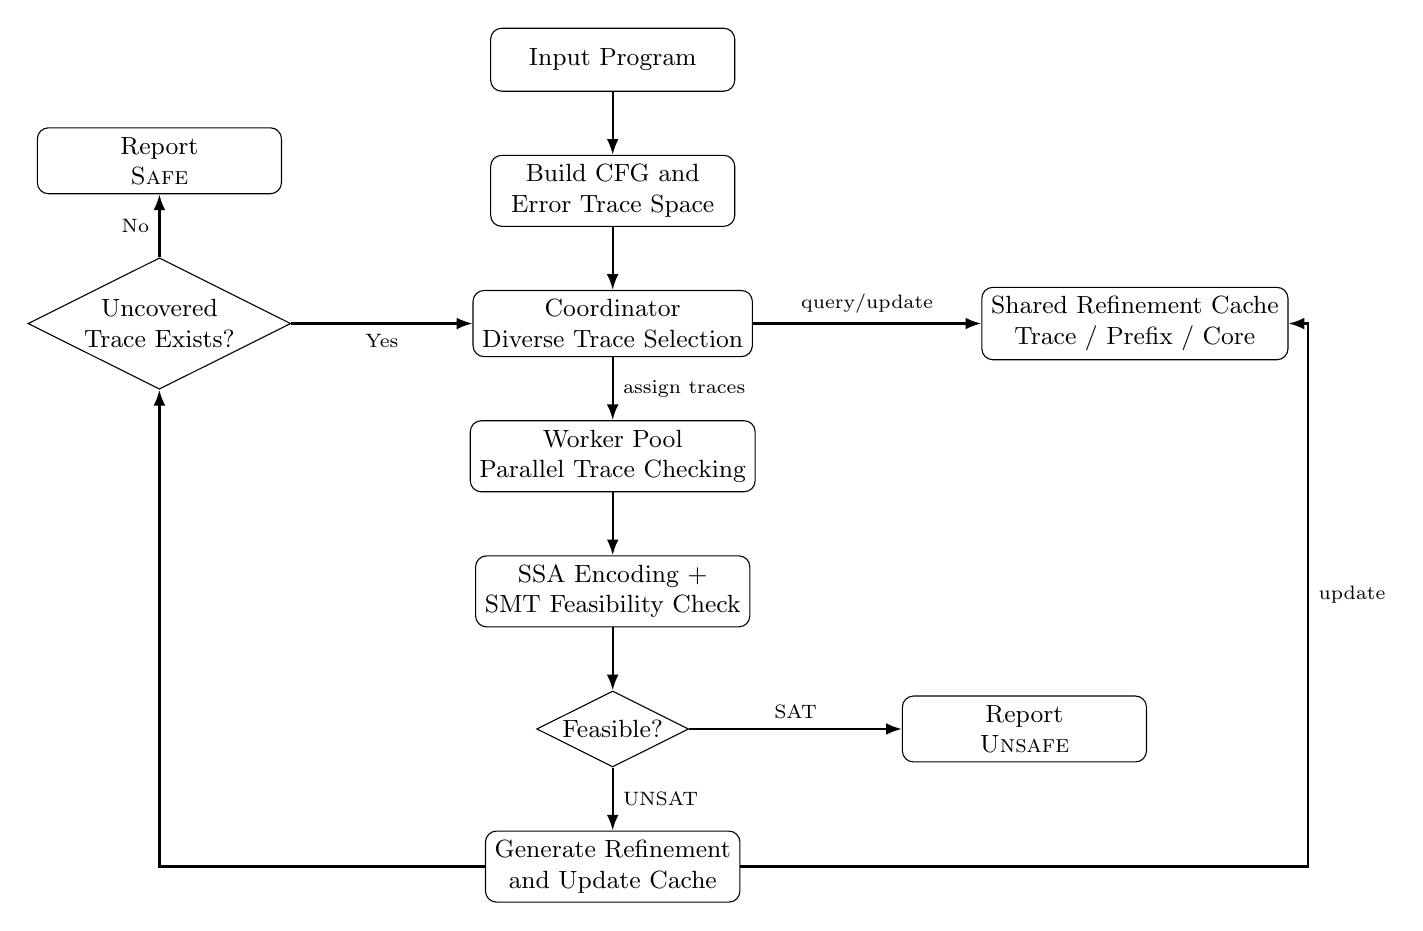
\begin{tikzpicture}[
    node distance=0.8cm and 0.9cm,
    process/.style={
        rectangle,
        rounded corners,
        draw,
        align=center,
        minimum width=3.1cm,
        minimum height=0.8cm,
        font=\small
    },
    decision/.style={
        diamond,
        draw,
        align=center,
        aspect=2,
        inner sep=1pt,
        font=\small
    },
    arrow/.style={-{Latex[length=2mm]}, thick}
]
\node[process] (program) {Input Program};
\node[process, below=of program] (cfg) {Build CFG and\\Error Trace Space};
\node[process, below=of cfg] (coord) {Coordinator\\Diverse Trace Selection};
\node[process, right=of coord, xshift=2.0cm] (cache) {Shared Refinement Cache\\Trace / Prefix / Core};
\node[process, below=of coord] (workers) {Worker Pool\\Parallel Trace Checking};
\node[process, below=of workers] (smt) {SSA Encoding +\\SMT Feasibility Check};
\node[decision, below=of smt] (feasible) {Feasible?};
\node[process, right=of feasible, xshift=1.8cm] (unsafe) {Report\\\textsc{Unsafe}};
\node[process, below=of feasible] (refine) {Generate Refinement\\and Update Cache};
\node[decision, left=of coord, xshift=-1.4cm] (empty) {Uncovered\\Trace Exists?};
\node[process, above=of empty] (safe) {Report\\\textsc{Safe}};

\draw[arrow] (program) -- (cfg);
\draw[arrow] (cfg) -- (coord);
\draw[arrow] (coord) -- node[above, font=\scriptsize] {query/update} (cache);
\draw[arrow] (coord) -- node[right, font=\scriptsize] {assign traces} (workers);
\draw[arrow] (workers) -- (smt);
\draw[arrow] (smt) -- (feasible);
\draw[arrow] (feasible) -- node[above, font=\scriptsize] {SAT} (unsafe);
\draw[arrow] (feasible) -- node[right, font=\scriptsize] {UNSAT} (refine);

\draw[arrow] (refine.east) -| node[pos=0.75, right, font=\scriptsize] {update} ([xshift=0.25cm]cache.east) -- (cache.east);

\draw[arrow] (refine.west) -| (empty.south);

\draw[arrow] (empty.east) -- node[below, font=\scriptsize] {Yes} (coord.west);

\draw[arrow] (empty) -- node[left, font=\scriptsize] {No} (safe);
\end{tikzpicture}
\caption{Refinement-aware parallel CEGAR workflow. The coordinator selects diverse uncovered traces, workers check them in parallel, and learned refinements are shared through a cache to prune future work.}
\label{fig:parallel-refinement-flow}
\end{figure}

\begin{table}[h]
\centering
\small
\begin{tabular}{|l|l|l|}
\hline
\textbf{Configuration} & \textbf{Trace Selection} & \textbf{Refinement Sharing} \\
\hline
SEQ & BFS, one trace at a time & Local refinement only \\
\hline
PAR-Basic & BFS with multiple workers & Exact trace blocking \\
\hline
PAR-Diverse & Early-divergence selection & Exact trace blocking \\
\hline
PAR-Cache & BFS with cache filtering & Trace and prefix cache \\
\hline
PAR-Diverse-Cache & Diverse and cache-aware selection & Trace, prefix, and optional unsat-core cache \\
\hline
\end{tabular}
\caption{Planned configurations for studying the effect of trace diversity and shared refinement information.}
\label{tab:configs}
\end{table}

\section*{4. Evaluation}
The proposed framework will be evaluated on two benchmark sets. First, we will use a small public benchmark subset adapted from SV-COMP/SV-Benchmarks, following the experimental setting of prior work on parallel trace abstraction. We will focus on sequential C reachability tasks with the \texttt{unreach-call} property and select programs whose core behavior can be represented in our simplified imperative language, such as integer variables, branches, bounded loops, and assertions. This subset provides a more credible comparison source without requiring a full C frontend.

Second, we will construct controlled synthetic benchmarks to isolate the effects of trace diversity and shared refinement caching. These benchmarks will vary the number of branches, trace depth, amount of shared infeasible prefixes, ratio of feasible to infeasible traces, and overlap among spurious counterexamples. We will compare the configurations in Table~\ref{tab:configs} using different worker counts, such as 1, 2, 4, and 8 workers.

The primary metrics are wall-clock execution time, number of SMT queries, number of traces skipped by the cache, cache hit rate, number of refinements, and redundant work ratio. We will also measure cases where parallelization hurts due to synchronization overhead or poor trace selection. The evaluation will be considered successful if it identifies when diverse trace selection and shared refinement caching reduce redundant SMT work and improve response time, especially on benchmarks with many overlapping spurious traces.

\end{document}
